\subsubsection{UC 5 - Creazione di una prenotazione}

\begin{figure}[h]
  \centering
    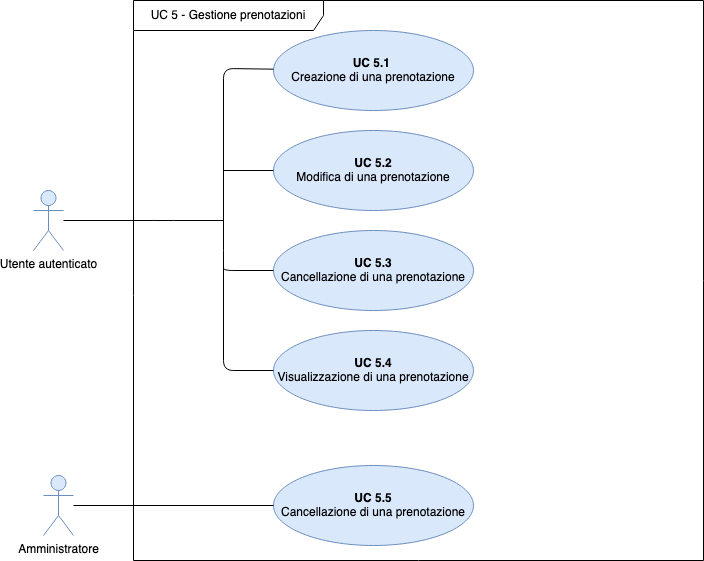
\includegraphics[scale=0.5]{src/CasiDUso/Immagini/UC5.png}
  \caption{UC5  - Creazione di una prenotazione}
\end{figure}

Il presente diagramma vuole riassumere la possibilità di gestione delle prenotazioni da parte di un utente autenticato nell’applicazione.

\begin{itemize}
\item \textbf{Attori primari:} utente autenticato;
\item \textbf{Descrizione:} l’utente vuole gestire una prenotazione a cui ha accesso a livello di permessi, con possibilità di creazione, modifica, eliminazione e visualizzazione;
\item \textbf{Precondizione:} l’utente è autenticato nell’applicazione e ha i permessi per eseguire le azioni di cui sopra;
\item \textbf{Postcondizione:} l’utente ha creato, modificato, eliminato o visualizzato una prenotazione;
\item \textbf{Scenario principale:} 
	\begin{itemize}
		\item l’utente naviga nell’apposita sezione di modifica della prenotazione;
		\item l’utente crea, visualizza, modifica o rimuove una sua prenotazione;
		\item la prenotazione passa in stato di “pending” e, dopo una serie di controlli, viene confermata o eliminata.
	\end{itemize}
\end{itemize}

\subsubsection{UC5.1 - Creazione di una prenotazione}

\begin{itemize}
\item \textbf{Attori primari:} utente autenticato;
\item \textbf{Descrizione:} l’utente vuole prenotare una postazione per una certa data od orario;
\item \textbf{Precondizione:} l’utente è autenticato e naviga nell’apposita sezione di creazione di una prenotazione;
\item \textbf{Postcondizione:} l’utente crea correttamente una prenotazione per la data ed ora scelta;
\item \textbf{Scenario principale:} 
	\begin{itemize}
		\item il sistema elabora correttamente la richiesta, mandando in stato di “pending” la prenotazione;
		\item il sistema restituisce un errore per i seguenti motivi:
		\begin{itemize}
			\item la postazione è già stata prenotata per quella determinata fascia oraria;
			\item la postazione è stata disabilitata da un amministratore di sistema.	
		\end{itemize}
	\end{itemize}
\end{itemize}

\subsubsection{UC5.2 - Modifica di una prenotazione}

\begin{itemize}
\item \textbf{Attori primari:} utente autenticato;
\item \textbf{Descrizione:} l’utente vuole modificare una postazione per una certa data od orario;
\item \textbf{Precondizione:} l’utente è autenticato e naviga nell’apposita sezione di modifica di una prenotazione;
\item \textbf{Postcondizione:} l’utente modifica correttamente una prenotazione per la nuova data/ora scelta;
\item \textbf{Scenario principale:} 
	\begin{itemize}
		\item il sistema elabora correttamente la richiesta, mandando in stato di “pending” la prenotazione;
		\item il sistema restituisce un errore per i seguenti motivi:
		\begin{itemize}
			\item la postazione è già stata prenotata per quella determinata fascia oraria;
			\item la postazione è stata disabilitata da un amministratore di sistema.	
		\end{itemize}
	\end{itemize}
\end{itemize}

\subsubsection{UC5.3 - Cancellazione di una prenotazione}

\begin{itemize}
\item \textbf{Attori primari:} utente autenticato;
\item \textbf{Descrizione:} l’utente vuole cancellare una prenotazione per una certa data od orario effettuata in precedenza;
\item \textbf{Precondizione:} l’utente è autenticato e naviga nell’apposita sezione di cancellazione di una prenotazione;
\item \textbf{Postcondizione:} l’utente cancella correttamente la prenotazione per la data/ora scelta;
\item \textbf{Scenario principale:} 
	\begin{itemize}
		\item il sistema elabora correttamente la richiesta;
		\item il sistema restituisce un errore per i seguenti motivi:
		\begin{itemize}
			\item non è possibile cancellare una prenotazione per un orario passato.
		\end{itemize}
	\end{itemize}
\end{itemize}

\subsubsection{UC5.4 - Visualizzazione di una prenotazione}

\begin{itemize}
\item \textbf{Attori primari:} utente autenticato;
\item \textbf{Descrizione:} l’utente vuole visualizzare le sue prenotazioni attive nel sistema;
\item \textbf{Precondizione:} l’utente è autenticato e naviga nell’apposita sezione di visualizzazione delle sue prenotazione;
\item \textbf{Postcondizione:} l’utente visualizza correttamente le sue prenotazioni attive;
\item \textbf{Scenario principale:} 
	\begin{itemize}
		\item il sistema elabora correttamente la richiesta;
		\item il sistema restituisce un errore per i seguenti motivi:
		\begin{itemize}
			\item non si ha alcuna prenotazione attiva.
		\end{itemize}
	\end{itemize}
\end{itemize}

\subsubsection{UC5.5 - Cancellazione di una prenotazione}

\begin{itemize}
\item \textbf{Attori primari:} amministratore;
\item \textbf{Descrizione:} l’amministratore vuole impedire la prenotazione di una specifica postazione da parte di utenti autenticati;
\item \textbf{Precondizione:} l’amministratore è autenticato e naviga nell’apposita sezione di blocco prenotazione di una postazione;
\item \textbf{Postcondizione:} l’amministratore blocca correttamente la possibilità di prenotare una postazione per qualsiasi utente autenticato;
\item \textbf{Scenario principale:} 
	\begin{itemize}
		\item il sistema elabora correttamente la richiesta;
		\end{itemize}
\end{itemize}
